\documentclass{llncs}
\input{glyphtounicode}
\pdfgentounicode=1
\usepackage{graphicx,booktabs,tabularx,amsmath,amssymb}
\usepackage{accsupp}
\usepackage[hidelinks]{hyperref}
\hypersetup{pdfauthor={},pdftitle={Graph Representations for Congestion Onset Prediction: A Controlled Comparative Study}}
\newcommand{\TestOnAG}{0.01602}
\newcommand{\TestAllAG}{0.02060}
\newcommand{\TestCalOnAG}{0.01397}
\newcommand{\TestCalAllAG}{0.01874}
\newcommand{\TestRecallAG}{93.46\%}
\newcommand{\TestFprAG}{4.87\%}
\newcommand{\TestOnRUnion}{0.01425}
\newcommand{\TestAllRUnion}{0.01852}
\newcommand{\TestCalOnRUnion}{0.01286}
\newcommand{\TestCalAllRUnion}{0.01712}
\newcommand{\TestRecallRUnion}{96.15\%}
\newcommand{\TestFprRUnion}{5.29\%}
\newcommand{\TestOnAMono}{0.01467}
\newcommand{\TestAllAMono}{0.01920}
\newcommand{\TestCalOnAMono}{0.01381}
\newcommand{\TestCalAllAMono}{0.01870}
\newcommand{\TestRecallAMono}{93.46\%}
\newcommand{\TestFprAMono}{4.87\%}
\newcommand{\TestOnB}{0.01521}
\newcommand{\TestAllB}{0.01974}
\newcommand{\TestCalOnB}{0.01399}
\newcommand{\TestCalAllB}{0.01923}
\newcommand{\TestRecallB}{92.82\%}
\newcommand{\TestFprB}{5.97\%}
\newcommand{\TestOnK}{0.01535}
\newcommand{\TestAllK}{0.01993}
\newcommand{\TestCalOnK}{0.01412}
\newcommand{\TestCalAllK}{0.01960}
\newcommand{\TestRecallK}{93.21\%}
\newcommand{\TestFprK}{5.84\%}
\newcommand{\TestOnC}{0.01537}
\newcommand{\TestAllC}{0.01985}
\newcommand{\TestCalOnC}{0.01406}
\newcommand{\TestCalAllC}{0.01907}
\newcommand{\TestRecallC}{93.21\%}
\newcommand{\TestFprC}{6.32\%}
\newcommand{\TestOnD}{0.01515}
\newcommand{\TestAllD}{0.01979}
\newcommand{\TestCalOnD}{0.01399}
\newcommand{\TestCalAllD}{0.01949}
\newcommand{\TestRecallD}{92.82\%}
\newcommand{\TestFprD}{6.69\%}
\newcommand{\TestOnM}{0.01512}
\newcommand{\TestAllM}{0.01978}
\newcommand{\TestCalOnM}{0.01381}
\newcommand{\TestCalAllM}{0.01964}
\newcommand{\TestRecallM}{92.44\%}
\newcommand{\TestFprM}{4.94\%}
\newcommand{\TestOnS}{0.01524}
\newcommand{\TestAllS}{0.01983}
\newcommand{\TestCalOnS}{0.01386}
\newcommand{\TestCalAllS}{0.01949}
\newcommand{\TestRecallS}{92.82\%}
\newcommand{\TestFprS}{5.07\%}
\newcommand{\TestOnE}{0.01504}
\newcommand{\TestAllE}{0.01973}
\newcommand{\TestCalOnE}{0.01399}
\newcommand{\TestCalAllE}{0.01959}
\newcommand{\TestRecallE}{92.82\%}
\newcommand{\TestFprE}{7.12\%}
\newcommand{\TestOnF}{0.01538}
\newcommand{\TestAllF}{0.01986}
\newcommand{\TestCalOnF}{0.01418}
\newcommand{\TestCalAllF}{0.01916}
\newcommand{\TestRecallF}{92.69\%}
\newcommand{\TestFprF}{6.39\%}
\newcommand{\ValOnAG}{0.01411}
\newcommand{\ValAllAG}{0.01862}
\newcommand{\ValCalOnAG}{0.01425}
\newcommand{\ValCalAllAG}{0.01852}
\newcommand{\ValRecallAG}{92.39\%}
\newcommand{\ValFprAG}{4.05\%}
\newcommand{\ValOnRUnion}{0.01217}
\newcommand{\ValAllRUnion}{0.01605}
\newcommand{\ValCalOnRUnion}{0.01219}
\newcommand{\ValCalAllRUnion}{0.01621}
\newcommand{\ValRecallRUnion}{96.19\%}
\newcommand{\ValFprRUnion}{4.29\%}
\newcommand{\ValOnAMono}{0.01360}
\newcommand{\ValAllAMono}{0.01793}
\newcommand{\ValCalOnAMono}{0.01437}
\newcommand{\ValCalAllAMono}{0.01872}
\newcommand{\ValRecallAMono}{92.39\%}
\newcommand{\ValFprAMono}{4.05\%}
\newcommand{\ValOnB}{0.01217}
\newcommand{\ValAllB}{0.01704}
\newcommand{\ValCalOnB}{0.01269}
\newcommand{\ValCalAllB}{0.01870}
\newcommand{\ValRecallB}{97.00\%}
\newcommand{\ValFprB}{4.06\%}
\newcommand{\ValOnK}{0.01316}
\newcommand{\ValAllK}{0.01784}
\newcommand{\ValCalOnK}{0.01351}
\newcommand{\ValCalAllK}{0.01933}
\newcommand{\ValRecallK}{95.85\%}
\newcommand{\ValFprK}{4.16\%}
\newcommand{\ValOnC}{0.01240}
\newcommand{\ValAllC}{0.01713}
\newcommand{\ValCalOnC}{0.01284}
\newcommand{\ValCalAllC}{0.01836}
\newcommand{\ValRecallC}{97.58\%}
\newcommand{\ValFprC}{4.45\%}
\newcommand{\ValOnD}{0.01253}
\newcommand{\ValAllD}{0.01740}
\newcommand{\ValCalOnD}{0.01298}
\newcommand{\ValCalAllD}{0.01907}
\newcommand{\ValRecallD}{97.00\%}
\newcommand{\ValFprD}{4.42\%}
\newcommand{\ValOnM}{0.01317}
\newcommand{\ValAllM}{0.01781}
\newcommand{\ValCalOnM}{0.01360}
\newcommand{\ValCalAllM}{0.01959}
\newcommand{\ValRecallM}{95.85\%}
\newcommand{\ValFprM}{3.57\%}
\newcommand{\ValOnS}{0.01308}
\newcommand{\ValAllS}{0.01767}
\newcommand{\ValCalOnS}{0.01348}
\newcommand{\ValCalAllS}{0.01932}
\newcommand{\ValRecallS}{96.42\%}
\newcommand{\ValFprS}{3.82\%}
\newcommand{\ValOnE}{0.01228}
\newcommand{\ValAllE}{0.01743}
\newcommand{\ValCalOnE}{0.01281}
\newcommand{\ValCalAllE}{0.01930}
\newcommand{\ValRecallE}{97.00\%}
\newcommand{\ValFprE}{5.31\%}
\newcommand{\ValOnF}{0.01214}
\newcommand{\ValAllF}{0.01700}
\newcommand{\ValCalOnF}{0.01260}
\newcommand{\ValCalAllF}{0.01835}
\newcommand{\ValRecallF}{97.46\%}
\newcommand{\ValFprF}{4.33\%}
\newcommand{\TestOnsetN}{9,315}
\newcommand{\TestPos}{260}
\newcommand{\TestEligible}{10,327}
\newcommand{\TestPrevalence}{2.79\%}
\newcommand{\NewGPU}{35.50}
\newcommand{\CumulativeGPU}{1033.33}

\newcommand{\figalt}[2]{\BeginAccSupp{method=escape,ActualText={#1}}#2\EndAccSupp{}}
\begin{document}
\title{Graph Representations for Congestion Onset Prediction: A Controlled Comparative Study}
\author{Anonymous submission}
\institute{}
\maketitle
\begin{abstract}
Regional traffic risk predictors can retain individual sensor histories or summarize them before prediction. Graph operations provide several ways to use the same measurements, but improvements can also arise from stronger aggregate fitting or later training labels. We compare six compact temporal and graph representations against aggregate refitting, monotone recalibration, and matched residual controls for a sustained low-speed onset event in PEMS-BAY. Training choices precede an exposed validation period and a frozen chronological test evaluation. The test includes \TestOnsetN{} onset-eligible origins and \TestPos{} positives on 25 days. Aggregate refitting achieves onset Brier \TestOnRUnion{}, compared with \TestOnB{} for aggregate correction, \TestOnC{} for local histories, \TestOnD{} for distance messages, and \TestOnE{} for separate within-region and cross-region messages. Local histories alone remain worse than aggregate correction. Favorable graph point estimates do not exclude zero under the primary three-day, four-contrast adjustment. Cross-region messages beat both trained rewired controls in secondary comparisons, while increasing false alarms. These results support a controlled account of representation and baseline dependence, rather than a general claim that graphs help or are unnecessary. Weak calibration support and unresolved upstream preprocessing limit interpretation.
\keywords{Traffic forecasting \and Congestion onset \and Graph representations \and Aggregate baselines \and Chronological evaluation}
\end{abstract}

\section{Introduction}
A regional traffic digital twin must decide what to retain from a sensor network. Individual histories contain local differences that disappear in regional summaries. A graph can mix those histories according to geographic proximity or statistical association. Neither additional detail nor graph processing guarantees a better fitted predictor. A regional event may already be well described by aggregate slowing, heterogeneity, and calendar patterns. More recent labeled examples can also improve a baseline without requiring additional sensor-level inputs.

This study examines those alternatives for congestion onset prediction. The target is a sustained network-wide low-speed event over a short future horizon, rather than mean future speed at each detector. This distinction matters. A representation that improves a sensor-level regression objective need not improve an aggregate binary event, and a lower probability loss need not yield better alarms at an operational cutoff. We ask four questions. Do individual sensor histories improve prediction beyond rich aggregate histories? Does the particular graph structure help when local measurements are held fixed? How do geographic, regional, multiscale, cross-region, and dependency representations differ for this target? Do their differences translate into useful alarms and justified processing costs?

Our experiments use an unchanged aggregate probability anchor and compact additive corrections. This common interface separates the inputs and graph operations while keeping much of the fitting procedure fixed. The aggregate controls include refitting on the union of the anchor and correction training examples. That control, denoted $R_{\rm union}$, addresses a basic confound: comparing a predictor trained on older, fewer labels with a correction trained later can overstate the value of its additional inputs. A larger aggregate correction also checks whether local arms benefit simply from additional parameters.

The scope is deliberately comparative. We evaluate six representation families, three registered correction seeds, and trained topology controls. We do not present these models as complete reproductions of major traffic GNN architectures. The held-out period was opened only after committing the roster, artifact hashes, metrics, thresholds, and analysis. The paper retains unfavorable results and changes of direction between validation and test. Its contribution is evidence about a specified regional risk task under controlled fitting and information comparisons, together with a recoverable evaluation package. It is not a new residual-learning algorithm, a proof of aggregation sufficiency, or a claim that a negative result alone establishes novelty.

\section{Related Work}
Graph-based traffic forecasting combines temporal history with a spatial dependency model. DCRNN uses bidirectional diffusion and recurrent forecasting \cite{dcrnn}. Graph WaveNet combines temporal convolutions with an adjacency learned through node embeddings \cite{gwnet}. These methods motivate testing both fixed and measurement-derived connectivity. Our distance and dependency arms are much smaller controlled variants and predict a regional event probability directly. Their results cannot rank the original architectures on their established speed-forecasting benchmarks.

The need for strong simple spatial baselines is already documented. \emph{Do We Really Need Graph Neural Networks for Traffic Forecasting?} introduces SimST, which models local proximity and global correlations without conventional message passing \cite{simst}. STID uses spatial and temporal identity information with MLPs \cite{stid}. These studies show why comparing a graph model only with a weak nonspatial predictor is insufficient. Our local encoder retains regional identity and ordered histories, but is not a reproduction of SimST or STID. The additional question here is whether local and graph inputs help a rich aggregate event predictor after matching access to later labels.

Standardized evaluation is equally relevant. BasicTS+ examines inconsistent multivariate forecasting comparisons and supplies a common training pipeline \cite{basicts}. LargeST provides a broader traffic-flow benchmark \cite{largest}. We use neither their full model roster nor their standard scoring task. We retain one existing speed dataset and an explicitly defined chronological risk endpoint. The graph benchmarking framework of Dwivedi et al. motivates parameter-budget controls and reproducible comparison \cite{benchmark}; comparable parameter counts do not make different representations equally expressive.

Residual correction also has direct traffic precedents. ResCAL estimates errors of existing forecasts from previous errors and graph signals \cite{rescal}. Our corrections instead learn a bounded additive change to a frozen event probability from histories and summaries. Residual learning itself is established, and this input/target difference does not establish priority. We evaluate whether the mechanism is useful relative to aggregate updating.

Graph aggregation provides an analytical language for describing lost detail. Equitable partitions and quotient dynamics have established conditions under which grouped states close under an operator \cite{schaub}. Diffusion wavelets develop multiscale representations of diffusion operators \cite{diffusion}. The decomposition used below is elementary projection algebra. We use it to define candidate summaries, without claiming a new coarsening theorem or sufficiency for nonlinear congestion events.

\section{Task and Observation Model}
\subsection{Recorded-Speed Event and Onset Eligibility}
PEMS-BAY contains five-minute recorded speeds for 325 ordered sensors from January through June 2017 \cite{dcrnn,release}. The stored units are mph. Let $v_{i,t}$ be recorded speed and $f_i$ the fixed reference free speed, estimated as the 85th percentile within the original training period. For a fully observed frame, define
\begin{equation}
 c_t=\sum_{i=1}^{325}\mathbf{1}\{v_{i,t}\leq f_i/2\},\qquad
 Y_t=\mathbf{1}\!\left\{\max_{j=1,\ldots,4}\min_{k=0,1,2}c_{t+j+k}\geq48\right\}.
\label{eq:target}
\end{equation}
The predictor uses 12 frames ending at $t$ and estimates whether this event occurs within the next six frames. The onset population excludes origins already satisfying the three-frame current event rule. Thus onset denotes a prediction made while the sustained event is not currently known or possibly active. It is not a detector-level onset time or a road-incident annotation.

Nonfinite and nonpositive observations are treated as unknown. At each future frame, the lower count treats unknown sensors as not severe and the upper count treats them as severe. Applying Eq.~\ref{eq:target} to these counts gives lower and upper event labels. A forecast origin is scoreable only when these labels agree and at least 95\% of its future sensor-frame entries are observed. We do not impute missing future speeds into observed labels. For current onset eligibility, an unknown sensor is conservatively allowed to be severe, excluding a possibly active event. Every arm uses the same resulting masks.

This definition targets a recorded sustained low-speed condition. It does not establish that a particular incident occurred, that congestion propagated causally along an edge, or that an alarm would lead to a beneficial intervention. Those claims would require additional observations and an operational study.

\subsection{Aggregate and Local Inputs}
Sensors are assigned to 16 fixed regions by a deterministic recursive partition of coordinates. The aggregate vector has 1,158 entries: 12-frame histories of regional means and valid counts, six calendar terms, and histories of regional variance, minimum, maximum, and severe fraction. Summaries therefore preserve substantial heterogeneity as well as average slowing. Computing them already reads every sensor. They should not be described as saving sensor acquisition.

Feature speeds use an earlier-training reference and the clipped transformation
\begin{equation}
 x_{i,t}=\operatorname{logit}\!\left(\operatorname{clip}_{[.001,\allowbreak .999]}(1-v_{i,t}/f_i^{\rm feature})\right).
\end{equation}
Feature references and the historical target references have distinct fit cutoffs. Missing transformed entries contribute zero with explicit masks and valid counts. The aggregate correction input is standardized with the correction-training mean and scale, then clipped to $[-10,10]$.

Local arms receive each sensor's ordered transformed history, deviation from its regional mean, recent change when both frames are valid, and a validity channel. Shared temporal MLP parameters encode these histories. Masked pooling produces one vector for each fixed region, with regional availability fractions. Ordered regional outputs retain regional identity even without graph messages. Local arms add measurement detail to the aggregate vector; changing D to another graph with the same histories changes the inductive bias applied to those measurements.

\begin{figure}[t]
\centering
\figalt{A common sensor history supplies regional summaries and local representations. An aggregate anchor and one frozen correction produce a sustained-event probability.}{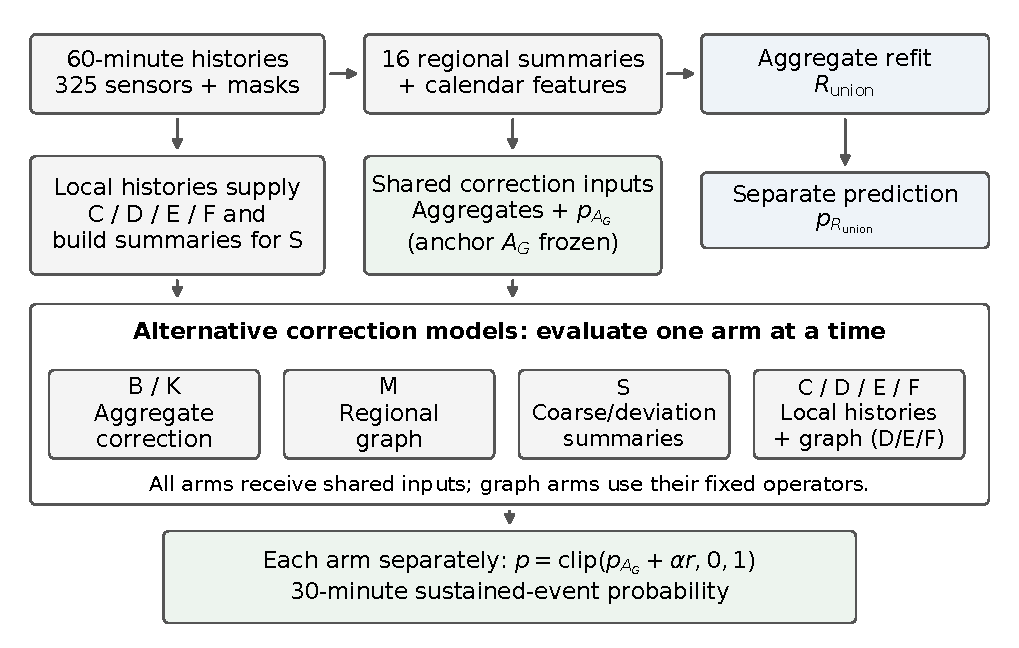
\includegraphics[width=\textwidth]{figures/overview.pdf}}
\caption{Controlled representation interface. All initial regional summaries require all-sensor ingestion. Local and graph branches add different representations of those histories; the graph is not a causal traffic-flow model.}
\label{fig:overview}
\end{figure}

\section{Predictors and Graph Representations}
\subsection{Frozen Anchor and Aggregate Controls}
The anchor $A_G$ is a GPU quantile-binned tree booster with 100 trees, at most 15 leaves, 64 candidate bins, minimum leaf size 20, and learning rate .1. Its L2 setting was selected from two choices within early training. $R_{\rm union}$ uses the same selected specification and feature transform, refitted on the exact union of the anchor and correction training examples at the same stride. Both have recoverable fitted weights. The earlier pilot's temporal baseline and a missing original sklearn fit are historical references only; saved probabilities do not reconstruct a fitted model.

$A_{\rm mono}$ applies a positive-slope logistic map to the frozen anchor. It was fitted on out-of-sample anchor predictions in the correction period. B adds a compact aggregate-only residual learner, and K increases the aggregate parameter budget to approximately that of local and graph corrections. The main-study training selection chose B as the aggregate comparator and E as the expanded graph comparator. These choices remain fixed for test, even when another arm has a better observed score.

Every correction uses
\begin{equation}
 p_t=\operatorname{clip}_{[0,1]}\{p_{A_G,t}+\alpha r_\theta(I_t)\},
 \qquad r_\theta(I_t)=\tfrac12\tanh g_\theta(I_t).
\label{eq:correction}
\end{equation}
The residual head was initialized to zero and trained using ordinary all-time Brier loss plus $\lambda r_\theta^2$, with weight decay. Zero correction recovers the anchor exactly. This property does not guarantee better generalization after fitting. A global $\alpha\in\{0,\allowbreak .25,\allowbreak .5,1\}$ was selected in a separate training block. It scales the residual before clipping. The frozen final evaluation changes none of these values.

\subsection{Six Representations}
Table~\ref{tab:inputs} summarizes the arms. C applies a shared MLP to each ordered local history and a self-message branch before masked regional pooling. D replaces that self message with one normalized weighted neighbor average. The original operator is a row-normalized distance-similarity matrix. Its weights indicate proximity, not verified directed road flow. The row convention determines which source histories a receiving node averages, without identifying causal direction.

M first encodes the available regional summary histories and exchanges messages on the fixed regional operator $Q=RWL$. It receives no extra local measurements. S instead exposes a small collection of graph-dependent regional summaries at hop scales one, two, and four. E uses separate within-region and cross-region messages, concatenated with each node's own encoding. Its two neighbor streams share the same total available-neighbor denominator. They are not independently renormalized to equal strength. E\_internal sets the cross-region stream to zero while retaining that denominator and the same architecture.

F substitutes a sparse training-estimated dependency operator into D's message architecture. Sensor histories are first residualized against earlier-training calendar terms and regional common components. Absolute residual correlations define neighbors, with each row's nonself degree matched to D. The retained association is unsigned, so negative associations also become positive averaging weights. F does not preserve all indegrees, optimize adjacency jointly with the forecast loss, or reveal causal road directions. These distinctions limit interpretations of either success or failure.

\begin{table}[t]
\caption{Main inputs and processing. Every correction also receives the aggregate vector and frozen anchor probability. Parameter counts exclude the shared anchor.}
\label{tab:inputs}
\small
\begin{tabularx}{\textwidth}{l l X r}
\toprule
Arm & Extra measurements & Representation & Parameters\\
\midrule
$A_G$, $R_{\rm union}$ & None & Aggregate tree predictors & Trees\\
$A_{\rm mono}$ & None & Monotone anchor map & 2\\
B & None & Aggregate correction & 38,209\\
K & None & Larger aggregate correction & 50,129\\
C & Full local histories & Shared temporal encoder, self message & 49,553\\
D & Full local histories & Distance-weighted sensor messages & 49,553\\
M & None & Messages among regional summaries & 49,937\\
S & Graph summaries & Coarse and deviation streams at 1, 2, 4 hops & 50,321\\
E & Full local histories & Separate internal and boundary messages & 49,809\\
F & Full local histories & Frozen sparse dependency messages & 49,553\\
\bottomrule
\end{tabularx}
\end{table}

The message and temporal widths are 16, and the ordinary aggregate and final hidden widths are 32. K uses aggregate width 42. All local and graph outputs pass through the same regional interface where feasible. Differences remain in input dimension, number of channels, normalization and effective function class. A matched parameter count is a capacity control, not a proof of equal optimization difficulty. B versus C therefore compares fitted representations and learning problems; it does not isolate an intrinsic information value independent of the learner.

\subsection{Coarse State and Graph-Dependent Detail}
Let $L\in\mathbb{R}^{325\times16}$ lift a regional vector to sensors and let $R\in\mathbb{R}^{16\times325}$ average each nonempty region, so $RL=I$. For a fully observed vector $x$, write
\begin{equation}
 z=Rx,\quad u=x-Lz,\quad Q=RWL,\quad s_h=RW^hu.
\end{equation}
Then
\begin{equation}
 RWx=Qz+s_1,\qquad RW^hx=(RW^hL)z+s_h.
\label{eq:decomposition}
\end{equation}
S supplies the coarse and deviation terms separately at the fixed hop scales. Repeated sparse products compute these features without materializing dense powers. In general $RW^hL$ differs from $Q^h$, since omitted deviations can affect subsequent regional averages.

The first deviation term vanishes for every vector exactly when $RW(I-LR)=0$, equivalently $RW=QR$. This follows by substituting $u=(I-LR)x$ and requiring the linear map to vanish for all $x$. It is an established closure condition, not a new theorem. Forward invariance $WL=LQ$ alone is insufficient for this implication with a general directed operator. Equitable-partition results require their stated symmetry or closure assumptions \cite{schaub}. Diffusion and coarsening constructions likewise do not establish that these summaries are sufficient for Eq.~\ref{eq:target} \cite{diffusion}.

Missingness needs a separate interpretation. S uses observed regional means and zero-fills unavailable deviations. Equivalently, unavailable values are completed by their observed regional mean before applying the fixed linear decomposition, with zero convention for an empty region. The identity describes that completed feature vector. It does not identify the actual missing speed or make an availability-normalized graph commute with fixed regional averaging. Availability fractions accompany the features, and missing future outcomes remain bounded rather than imputed.

\subsection{Topology Controls and Attribution}
D's identity control is the matched C architecture. E has its own self-message and internal-only controls. Two outcome-blind rewiring seeds generate trained competitors for D and E through directed double-edge swaps. Each null preserves nonself edge count, per-node in/outdegree, source-row weight multisets and diagonal fallbacks. It changes neighbor identity, geometry and regional mixing. Cross-region edge count rises from 1,130 in the original graph to 2,228 in each null. Thus a real-versus-null difference is not a clean test of geometry while holding regional structure fixed.

The two rewired graphs are fixed negative controls, not uniform samples from the full degree-constrained graph ensemble. They receive the same tuning allowance and all three training seeds. Training with a null graph is distinct from perturbing an already-trained graph at evaluation. The final stage uses only the existing trained controls. Earlier sensitivity checks do not justify claiming that these models generally ignore topology.

\section{Experimental Design}
\subsection{Chronology, Frozen Choices and Exposure}
The original split uses 108 complete training days through April 19, 36 validation days from April 20 to May 25, and 36 test days from May 26 to June 30. Incomplete March 12 is excluded from training. Input and outcome windows remain inside their split, with a two-sided 90-minute embargo at boundaries. Timestamps are naive in the release; a timezone convention is not asserted.

The main training pipeline separates six roles: anchor fitting through February 23; correction fitting from February 24 to March 16; early stopping from March 17 to 24; shrinkage and family selection from March 25 to April 1; calibration from April 2 to 9; and a final development gate from April 10 to 19. Windows crossing these boundaries are embargoed. All labels are observable before their role's cutoff. The anchor has 5,173 eligible fitting examples and the refit has 7,070. Correction training uses the later portion at stride three, matching its contribution to the refit's union. This addresses the older pilot's comparison between stride-12 early baseline training and denser later correction training.

Each correction family had two predeclared regularization choices, one tuning seed, and three retained seeds for the selected setting. AdamW used learning rate .001, weight decay .0001, batch size 256, at most 60 epochs and patience eight. Training minimized unweighted all-time Brier with residual regularization; selection used development onset Brier. No event weighting changed the probability estimand. Earlier rolling chronological evaluations are retained even when weak or unfavorable. Their overlaps and limited event counts prevent interpreting them as independent studies.

All validation days had been exposed during prior development. In an earlier pilot, onset was a favorable secondary endpoint. That observation motivated its registered primary role in the main graph comparison. The strengthened main comparison was less favorable to local information. We explicitly retain this history. It prevents retrospective relabeling of the earlier exploratory finding as a primary result.

The final test stage opened previously unexamined measurements only after the full protocol and verified implementation were committed. All required checkpoints were present. Their hashes, graph operators, transforms, shrinkage, calibration, thresholds and seed membership were fixed before access. No test outcome determined a fit, exclusion definition, threshold, representation or manuscript illustration. Test and validation are reported separately, without pooling their losses or event groups.

\subsection{Metrics, Uncertainty and Alarms}
Raw onset Brier is primary. Raw all-time Brier is secondary, and scores after frozen calibration are labeled separately. For each family we average the three seed-specific losses at each origin before temporal resampling. We do not average probabilities into an ensemble. Per-seed scores and their descriptive standard deviation remain available.

The registered raw onset comparison family is C minus B, D minus C, E minus D, and E minus B. Negative values favor the first arm. We use 2,000 paired calendar-block resamples with seed 20261007, three-day blocks as primary and one-day blocks as sensitivity. All origins in a selected day and their model/seed pairing remain together. Contiguous calendar segments are resampled separately, preserving gaps. Four-contrast Bonferroni percentile intervals use 98.75\% marginal coverage as an approximate familywise assessment. We also show pointwise 95\% intervals. These intervals condition on the fitted models and do not capture all training or development-selection uncertainty.

B versus $R_{\rm union}$ is a required secondary comparison. Graph-versus-aggregate and topology-control contrasts are descriptive, with pointwise intervals. F remains secondary regardless of its point rank. Practical scales carried forward from the protocol are a .0001 absolute and 1\% relative local benefit, or .00005 and .5\% graph benefit. Alarm tolerances are a recall loss of .02 or FPR increase of .01. These are pilot interpretation scales, not equivalence margins or a substitute for uncertainty.

Each predictor's positive-slope logistic calibrator was fitted on separate, out-of-sample training predictions. The calibration block contains only 30 onset-positive origins in five groups on four days. Strict alarms use $p>c$, where the frozen cutoff targets 5\% calibration FPR and excludes ties without jitter. The map is nondecreasing after endpoint clipping and cannot recover ranking among tied zeros. Test recall and FPR are measured, not assumed to inherit the calibration target.

Positive forecast groups merge origins separated by less than 30 minutes; a gap of at least 30 minutes starts a new group. A group is detected if any origin in it alarms. False-alarm groups use the same gap rule among alarmed non-event origins. These summaries account for repeated adjacent forecasts but do not turn groups into verified independent incidents. Event/non-event loss contributions, fixed-bin reliability and clipping diagnostics complement overall Brier.

\subsection{Computation and Verification}
All scientific numerics ran on one NVIDIA RTX 6000 Ada Generation GPU, including transformations, graph operations, predictions, metrics, resampling and verification. CPU work handled orchestration, parsing, serialization and rendering. The final stage used PyTorch 2.8.0 with CUDA 12.8 and driver 570.124.06. Active allocations were capped at 32 billion bytes. Existing measured costs were reused, without an additional timing campaign or CPU benchmark.

Before test access, every raw and calibrated validation prediction vector was replayed exactly from the frozen checkpoints. Guards, hashes, labels, masks, origin alignment and zero-correction recovery passed focused checks. The held-out run and identical replay used the same committed implementation. Predictions matched exactly; the largest numeric metric difference was $2.22\times10^{-16}$, below the predeclared $10^{-12}$ tolerance. This small reduction-level difference prevents claiming exact identity of all metrics. Reproduction establishes what computation ran, not predictive adequacy or formal floating-point certification.

\section{Results}
\subsection{Held-Out Support and Competitive Aggregate Controls}
The test has 10,333 timestamp-eligible origins, of which \TestEligible{} are scoreable. Six fail future coverage and none has disagreeing event bounds. There are 1,147 all-time positives. The onset population has \TestOnsetN{} origins and \TestPos{} positives, prevalence \TestPrevalence{}, grouped into 45 positive forecast groups on 25 days. Validation had 8,981 onset origins, 289 positives and 47 groups on 26 days. These differing populations are not combined.

\begin{table}[t]
\caption{Main-family Brier and frozen onset alarms. Correction entries average seed-specific scores. Validation is exposed development evidence. Calibrated test onset scores are separate from the raw primary endpoint.}
\label{tab:scores}
\centering\small
\begin{tabular}{lrrrrrr}
\toprule
 & Val. onset & Test onset & Test all & Test cal. & Recall & FPR\\
\midrule
$A_G$ & 0.01411 & 0.01602 & 0.02060 & 0.01397 & 93.5\% & 4.87\% \\
$R_{\rm union}$ & 0.01217 & 0.01425 & 0.01852 & 0.01286 & 96.2\% & 5.29\% \\
$A_{\rm mono}$ & 0.01360 & 0.01467 & 0.01920 & 0.01381 & 93.5\% & 4.87\% \\
B & 0.01217 & 0.01521 & 0.01974 & 0.01399 & 92.8\% & 5.97\% \\
K & 0.01316 & 0.01535 & 0.01993 & 0.01412 & 93.2\% & 5.84\% \\
C & 0.01240 & 0.01537 & 0.01985 & 0.01406 & 93.2\% & 6.32\% \\
D & 0.01253 & 0.01515 & 0.01979 & 0.01399 & 92.8\% & 6.69\% \\
M & 0.01317 & 0.01512 & 0.01978 & 0.01381 & 92.4\% & 4.94\% \\
S & 0.01308 & 0.01524 & 0.01983 & 0.01386 & 92.8\% & 5.07\% \\
E & 0.01228 & 0.01504 & 0.01973 & 0.01399 & 92.8\% & 7.12\% \\
F & 0.01214 & 0.01538 & 0.01986 & 0.01418 & 92.7\% & 6.39\% \\

\bottomrule
\end{tabular}
\end{table}

$R_{\rm union}$ has the lowest raw onset and all-time point scores among the main families, \TestOnRUnion{} and \TestAllRUnion{} (Table~\ref{tab:scores}). Its frozen-calibrated scores are also lowest, \TestCalOnRUnion{} and \TestCalAllRUnion{}. B's raw onset score is \TestOnB{}. The secondary difference of B minus $R_{\rm union}$ is .00096564. Its three-day pointwise interval is $[-.00000809,\allowbreak .00253475]$. This favors aggregate refitting in point estimate while remaining uncertain. It does not prove statistical superiority or equivalence. The corresponding validation difference was near zero. The refit remains an essential control because it has access to the same union of fitting labels without local histories.

$A_{\rm mono}$ reaches raw onset \TestOnAMono{}, showing that a simple training-fitted probability map also competes with the residual arms. ``Raw'' here means the arm's registered output before its additional final calibration map; $A_{\rm mono}$ is already a calibration control by construction. No score is relabeled as an uncalibrated simulator probability.

\subsection{Registered Representation Contrasts}
C remains worse than B on test. Its onset difference is +.00015935, or a 1.05\% relative increase, with adjusted three-day interval $[.00005218,\allowbreak .00023148]$. This direction persists from the strengthened validation comparison. It establishes a disadvantage for this fitted local representation, not zero information value of sensor histories.

D versus C changes direction from validation. Its test difference is -.00022027, a 1.43\% relative reduction. The pointwise interval $[-.00036401,\allowbreak -.00000627]$ favors D, but the adjusted three-day interval $[-.00043644,\allowbreak .00002676]$ crosses zero. E versus D is -.00010744, a .71\% reduction. Its adjusted interval is $[-.00023180,\allowbreak .00000729]$. This retains the favorable validation point direction but loses its adjusted exclusion of zero. E versus B reverses from an unfavorable validation point to -.00016836, or 1.11\%, on test. Its adjusted interval $[-.00029598,\allowbreak .00002452]$ also crosses zero.

\begin{figure}[t]
\centering
\figalt{Four paired Brier contrasts are shown separately for exposed validation and frozen test, for onset and all-time outcomes. C minus B stays positive, while several graph contrasts change direction or remain uncertain.}{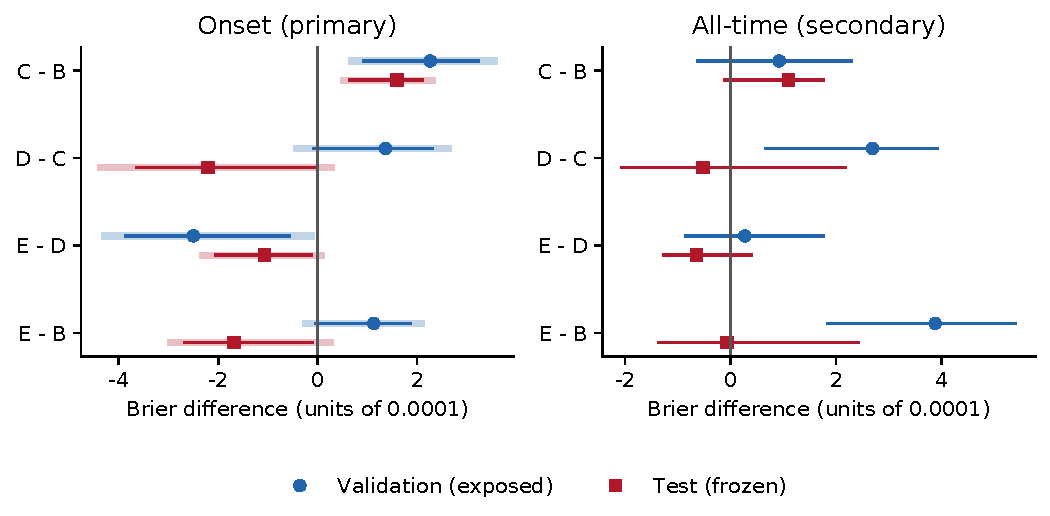
\includegraphics[width=\textwidth]{figures/effects.pdf}}
\caption{Paired endpoint effects. Thin intervals are pointwise three-day 95\%; pale thick onset intervals are the four-comparison adjusted intervals. Left favors the first named arm. Validation and test are separate evaluations.}
\label{fig:effects}
\end{figure}

The graph point differences exceed the carried-forward practical Brier scales, but uncertainty and alarms must be assessed separately. One-day adjusted intervals favor D over C and E over B, whereas the primary three-day adjusted intervals do not. This block-length sensitivity is visible evidence of temporal dependence, not a reason to promote the more favorable convention. Seed variation also remains. E improves over B in two seeds and worsens in the third. C is worse than B in all three test seeds. Agreement across three seeds would still not supply three independent realizations of the event process.

All-time effects are generally smaller among corrections and do not follow every onset ordering (Fig.~\ref{fig:effects}). E's all-time score is \TestAllE{}, compared with B's \TestAllB{} and $R_{\rm union}$'s \TestAllRUnion{}. F, the best validation onset point estimate among corrections, scores \TestOnF{} on test and is worse than B in a secondary pointwise comparison. F was never substituted for training-selected E. This reversal cautions against attributing its validation ranking to a generally superior dependency graph.

\subsection{Topology and Regional Representation}
E has the lowest raw onset point score among the six representations C through F. Regional-only M has score \TestOnM{}, while S has \TestOnS{}. These comparisons do not establish that local deviations are unnecessary, or that a multiscale feature design is intrinsically inferior. M and S have different inputs and processing paths, and their differences are small relative to temporal uncertainty.

D fails to beat both trained rewired controls. It is worse than rewiring seed 04 by .00004839, with pointwise interval $[.00001082,\allowbreak .00008544]$, while its comparison with seed 05 is uncertain. The particular distance topology therefore lacks consistent support in this architecture.

E provides a more favorable but qualified topology result. It beats both trained rewired controls on test by .00018858 and .00024918, with pointwise intervals $[-.00027045,\allowbreak -.00006917]$ and $[-.00041232,\allowbreak -.00004701]$. Both paired differences favor E in all three seeds. Its internal-only contrast is also favorable, while E versus E\_self remains uncertain. These are secondary comparisons, and the two real-versus-null directions were not consistently favorable on validation. Moreover, the nulls alter regional mixing. The evidence supports a limited statement about this trained within/cross-region representation and these controls, not a causal effect of road geometry.

\begin{figure}[t]
\centering
\figalt{Real versus trained null graph contrasts vary between validation and test. E beats both rewired controls on test, while D does not, and E versus its self control remains uncertain.}{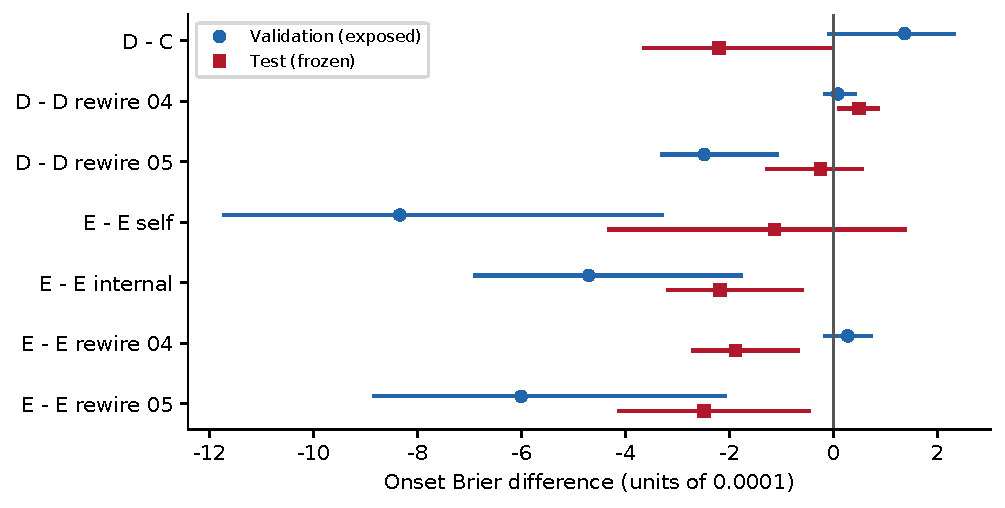
\includegraphics[width=\textwidth]{figures/topology.pdf}}
\caption{Existing trained topology controls, with pointwise three-day intervals. Nulls preserve degrees and row weights but change regional mixing. These descriptive contrasts are outside the adjusted primary family.}
\label{fig:topology}
\end{figure}

\subsection{Alarms, Calibration and Error Structure}
$R_{\rm union}$ achieves onset recall \TestRecallRUnion{} at FPR \TestFprRUnion{}. B, D and E share mean recall \TestRecallB{}, with FPR \TestFprB{}, \TestFprD{} and \TestFprE{}, respectively. E's FPR increase over B exceeds the registered one-percentage-point tolerance without a recall gain. Its favorable onset point Brier therefore does not yield an unqualified alarm improvement. $R_{\rm union}$ detects all 45 positive groups; B, C, D and E each detect an average of 43.33. Group detection is forgiving and should not be equated with every positive origin being detected.

\begin{figure}[t]
\centering
\figalt{Frozen test onset recall and false-alarm rates are plotted with three-day intervals. A second panel compares raw and frozen-calibrated reliability for aggregate refitting, aggregate correction and cross-region correction.}{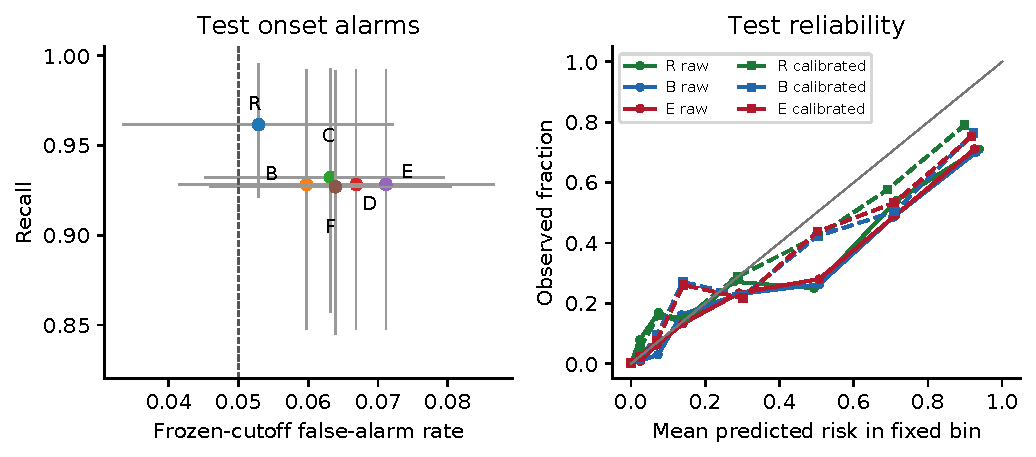
\includegraphics[width=\textwidth]{figures/alarms.pdf}}
\caption{Test alarm and calibration behavior. R denotes $R_{\rm union}$. The dashed vertical line is the training FPR target, not a test guarantee. Reliability bins pool seed-origin diagnostics without treating them as independent observations. Calibration does not select new thresholds.}
\label{fig:alarms}
\end{figure}

Frozen calibration improves test onset Brier for every main arm, reversing its adverse effect on validation. It leaves the observed alarm decisions unchanged here. $R_{\rm union}$'s calibrated onset score is \TestCalOnRUnion{}, compared with B \TestCalOnB{} and E \TestCalOnE{}. E no longer has a favorable calibrated point score relative to B. Calibration support is too limited to interpret this period-specific benefit as a general calibration guarantee.

Clipping remains substantial. B, C, D and E put approximately 86.61\%, 86.04\%, 85.78\% and 84.17\% of seed-origin onset predictions at exactly zero. M and S include a seed with a zero alarm cutoff. Positive monotone calibration moves a tied endpoint mass but cannot recreate within-mass ranking. No noise was added to resolve ties. The test's mean predicted onset probabilities exceed its prevalence for these principal corrections, and high-probability bins overpredict observed risk (Fig.~\ref{fig:alarms}). These are measured calibration diagnostics, not an explanation inferred solely from Brier.

For B, the event and non-event contributions to onset Brier are .00545291 and .00975926; for E they are .00559565 and .00944816. E reduces non-event loss but increases event loss. Its total improvement does not imply better recall. For each frozen arm, with $\delta=p-p_{A_G}$ after clipping, the evaluation verifies
\begin{equation}
 \overline{(Y-p_{A_G})^2-(Y-p)^2}
 =2\overline{\delta(Y-p_{A_G})}-\overline{\delta^2}.
\end{equation}
This established identity separates alignment with anchor errors from correction magnitude. It is descriptive algebra, not a novel explanation of generalization or a causal attribution to graph structure.

\subsection{Measured Costs}
Table~\ref{tab:cost} reuses the earlier complete inference workload of 128 timestamp-selected validation origins. It includes warm-cache HDF history parsing, transfers, feature preparation, the relevant predictor and output transfer. Model restoration and graph preparation were measured separately as shared setup. The three repeats use the first registered seed only. These costs do not include future-label creation and are not measurements of a deployed telemetry service.

\begin{table}[t]
\caption{Previously measured GPU fitting and complete 128-origin inference costs in seconds. Correction fitting lists the three selected seeds; tuning costs are recorded separately in the ledger. Inference means were summarized on CUDA from saved repeats.}
\label{tab:cost}
\centering\small
\begin{tabular}{lrrl}
\toprule
Arm & Selected fit(s) & Mean inference & Inference repeats\\
\midrule
$A_G$ & 2.363 & 0.2022 & 0.2124/0.1966/0.1976 \\
$R_{\rm union}$ & 2.699 & 0.2038 & 0.2136/0.1995/0.1984 \\
$A_{\rm mono}$ & n/a & 0.2074 & 0.2169/0.2074/0.1979 \\
B & 0.437/0.349/0.398 & 0.2066 & 0.2069/0.2188/0.1943 \\
K & 0.451/0.276/0.313 & 0.2061 & 0.2064/0.2101/0.2017 \\
C & 1.045/0.828/0.751 & 0.2087 & 0.2113/0.2079/0.2069 \\
D & 1.012/0.727/0.813 & 0.2080 & 0.2078/0.1999/0.2164 \\
M & 0.524/0.646/0.696 & 0.2052 & 0.1978/0.2095/0.2084 \\
S & 0.689/0.838/0.997 & 0.2048 & 0.2030/0.2054/0.2061 \\
E & 0.942/0.723/0.836 & 0.2066 & 0.2026/0.2078/0.2094 \\
F & 0.959/0.986/0.828 & 0.2068 & 0.2038/0.2061/0.2105 \\

\bottomrule
\end{tabular}
\end{table}

Complete costs are close across these compact arms, with overlapping measured repeats. We do not infer a reliable latency advantage from small ordering differences. The final stage consumed \NewGPU{} GPU-job seconds including startup, development replay, test evaluation and replay. Cumulative project usage is \CumulativeGPU{} seconds. CUDA event spans include host gaps and are not active-kernel totals. No new timing campaign, acquisition experiment or CPU benchmark was run.

Representation payload accounting is a specification, not measured communication savings. A float32 aggregate vector occupies 4,632 bytes before its other metadata. Full local histories add 15,600 value bytes, while three additional regional deviation-summary streams add 2,304. Masks, identifiers and shared graph metadata must also be counted. Both kinds of summary require all-sensor ingestion. The study establishes neither acquisition savings nor a measured reduction in stored or transmitted traffic data.

\section{Discussion and Limitations}
The local-history question has a narrow answer. C loses to aggregate correction B on both the strengthened validation comparison and the frozen test, with an adverse adjusted test interval. This does not show that local identity has no predictive information. C changes both representation and learning problem, while its temporal encoder, pooling, optimization and regularization restrict what can be learned. Rich regional extrema and severe fractions may already capture useful local behavior, but that is a plausible interpretation rather than a demonstrated sufficiency result.

The graph question has a different answer. D improves over C in test point estimate, but not under the primary three-day adjusted assessment, and it does not beat both trained rewired controls. E's cross-region representation has favorable secondary topology comparisons on test and the best raw onset point score among the six representations. That evidence coexists with uncertain primary intervals, a weaker validation null result and higher false alarms. It would be inaccurate either to claim a robust graph advantage over strong aggregates or to conclude that topology never matters.

Aggregate updating is the clearest competitive alternative. $R_{\rm union}$'s favorable point scores and alarm behavior survive the move to test without adding local inputs. Its comparison with B remains uncertain at the three-day scale, so the result is not a noninferiority proof. Nonetheless, a comparative study that omitted this control would give an incomplete account of the residual and graph mechanisms. More labels and a different fitting schedule can matter independently of access to graph detail.

Temporal support limits every conclusion. Overlapping forecast origins produce many labeled examples but relatively few event groups. A fixed 36-day test period supplies one chronological evaluation, not an independent sample of cities, seasons or incident types. Prior validation exposure influenced the research direction, and earlier rolling folds were small. The block bootstrap conditions on fitted models and uses a short series of day blocks. Its sensitivity to block length is an uncertainty limitation rather than a tuning opportunity.

Measurement provenance is also incomplete. The public DCRNN release documents access and window generation \cite{release}; its software license does not establish rights in the underlying measurements. The Caltrans source page documents a registration-based archive and historical reprocessing of speed estimates \cite{caltrans}. The exact detector-to-HDF cleaning, smoothing, imputation and processing version remain unresolved. Our masks and embargoes establish the behavior of this analysis, not the chronology or authenticity of every upstream transformation. No specific prohibition was identified and bypassed, but public availability alone does not establish analysis or redistribution permission. Raw speeds are not redistributed with this draft.

Finally, this is a bounded empirical comparison. It offers no new graph theorem, no claim of comprehensive traffic-model superiority, and no evidence for a telemetry policy. The failed simulator and uninformative enclosure campaign remain in the historical record but do not determine the graph conclusion. Exact-arithmetic projection or enclosure reasoning is distinct from floating-point certification, and passing implementation checks is distinct from an adequate predictive model. Publication readiness requires human scientific review, verified authorship and a resolved measurement-use path.

\section{Conclusion}
The frozen test evaluation preserves a disadvantage for the tested local-history correction and reveals modest, uncertain graph benefits relative to that correction. Separate within-region and cross-region messages beat the two existing trained rewired controls in secondary test comparisons, yet produce more false alarms and do not displace the aggregate refit. The strongest defensible contribution is a controlled, recoverable comparison showing how baseline label access, representation, topology controls and alarm calibration change the interpretation of congestion-onset results. These findings are specific to the target, dataset, fitted models and chronological period. The next step is independent scientific and provenance review of the comparative evidence, with no further optimization on this now-exposed test set.

\section*{AI Assistance and Draft Status}
An AI coding and writing assistant supported implementation, analysis orchestration, literature checking and manuscript drafting. The draft requires human verification and author approval before submission. No AI system is an author. No conference submission has been made.

\bibliographystyle{splncs04}
\bibliography{references}
\appendix
\section{Per-Seed Onset Results}
\begin{table}[h]
\caption{All frozen test arms. Corrections retain seeds 20261001, 20261002 and 20261003 in order. Null suffixes 04/05 identify graph seeds 20261004/20261005. SD is descriptive with denominator three, not a confidence interval.}
\centering\small
\begin{tabular}{lrrrr}
\toprule
Arm & Seed 01 & Seed 02 & Seed 03 & SD\\
\midrule
$A_G$ & 0.016018 & -- & -- & 0.000000 \\
$R_{\rm union}$ & 0.014247 & -- & -- & 0.000000 \\
$A_{\rm mono}$ & 0.014674 & -- & -- & 0.000000 \\
B & 0.015521 & 0.015031 & 0.015085 & 0.000220 \\
K & 0.015741 & 0.015297 & 0.015027 & 0.000294 \\
C & 0.015715 & 0.015171 & 0.015229 & 0.000244 \\
D & 0.015312 & 0.014845 & 0.015296 & 0.000217 \\
M & 0.015341 & 0.014823 & 0.015185 & 0.000217 \\
S & 0.015423 & 0.014899 & 0.015387 & 0.000239 \\
E & 0.015057 & 0.014757 & 0.015317 & 0.000229 \\
F & 0.015668 & 0.014971 & 0.015494 & 0.000296 \\
E\_internal & 0.015683 & 0.014834 & 0.015271 & 0.000347 \\
D rew. 04 & 0.015222 & 0.014739 & 0.015348 & 0.000263 \\
D rew. 05 & 0.015480 & 0.014859 & 0.015191 & 0.000253 \\
E\_self & 0.015299 & 0.014832 & 0.015342 & 0.000231 \\
E rew. 04 & 0.015328 & 0.014803 & 0.015566 & 0.000319 \\
E rew. 05 & 0.015662 & 0.014769 & 0.015448 & 0.000381 \\

\bottomrule
\end{tabular}
\end{table}
\end{document}
